\chapter{Looking into real-world data}
\addcontentsline{toc}{chapter}{Looking into real-world data}
\section{Five real-world stocks and their evolution over 15 years}
We have chosen to study five stocks listed on the Paris Stock Exchange : BNP Paribas, Carrefour, LVMH, Sanofi and Total stocks.\footnote{We have chosen companies positioned on different domains, otherwise, information from different stock might more easily be redundant.} The evolution of the stock prices has been studied over the past 15 years, on a weekly basis. We first draw the data itself, then the net returns and the gross log returns on the stocks\footnote{Both quantities are widely used in Finance.}
\begin{figure}[h!]
	\centering
	\begin{minipage}[b]{0.4\textwidth}
 	\centering
 	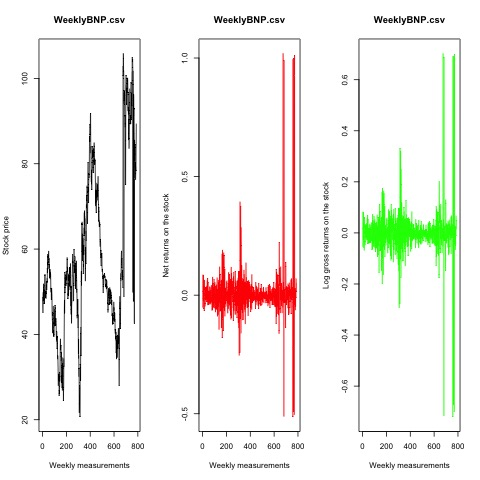
\includegraphics[scale = 0.4]{/Users/kimartin/Desktop/PDM_thesis_report/latex_template5_57/main/R_Files_3/WeeklyBNP.jpeg}
 	\caption{15 years of weekly BNP Stock Price Data}
 	\label{fig:BNPStock}
	\end{minipage}
	~
	\begin{minipage}[b]{0.4\textwidth}
  	\centering
  	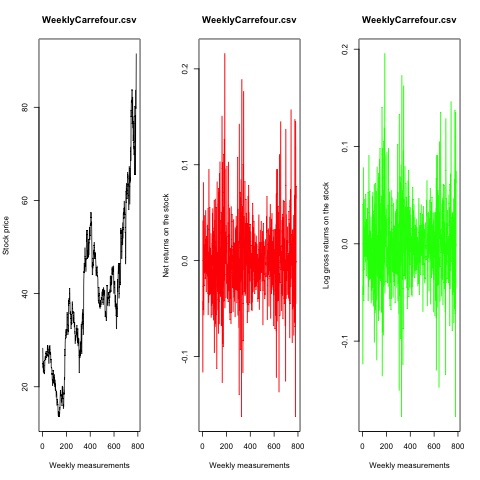
\includegraphics[scale = 0.4]{/Users/kimartin/Desktop/PDM_thesis_report/latex_template5_57/main/R_Files_3/WeeklyCarrefour.jpeg}
  	\caption{15 years of weekly Carrefour Stock Price Data}
  	\label{fig:CarrefourStock}
	\end{minipage}
\end{figure}
\begin{figure}[h!]
	\centering
	\begin{minipage}[b]{0.4\textwidth}
   	\centering
   	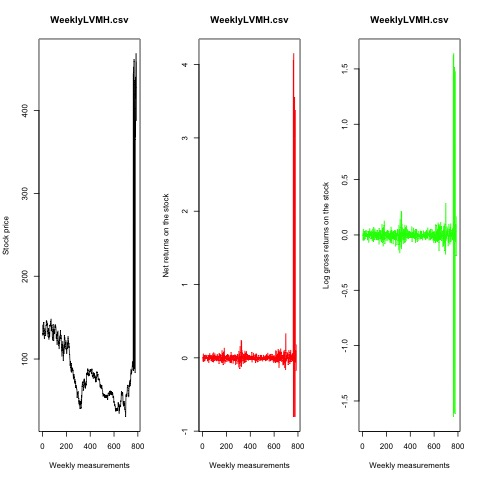
\includegraphics[scale = 0.4]{/Users/kimartin/Desktop/PDM_thesis_report/latex_template5_57/main/R_Files_3/WeeklyLVMH.jpeg}
   	\caption{15 years of weekly LVMH Stock Price Data}
   	\label{fig:LVMHStock}
	\end{minipage}
	~
	\begin{minipage}[b]{0.4\textwidth}
    	\centering
    	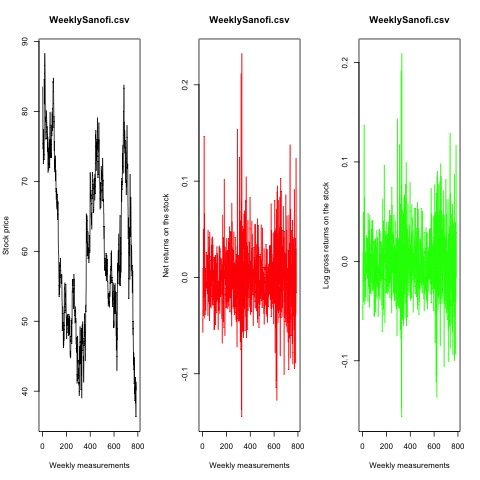
\includegraphics[scale = 0.4]{/Users/kimartin/Desktop/PDM_thesis_report/latex_template5_57/main/R_Files_3/WeeklySanofi.jpeg}
    	\caption{15 years of weekly Sanofi Stock Price Data}
    	\label{fig:SanofiStock}
	\end{minipage}
	~
	\begin{minipage}[b]{0.4\textwidth}
     	\centering
     	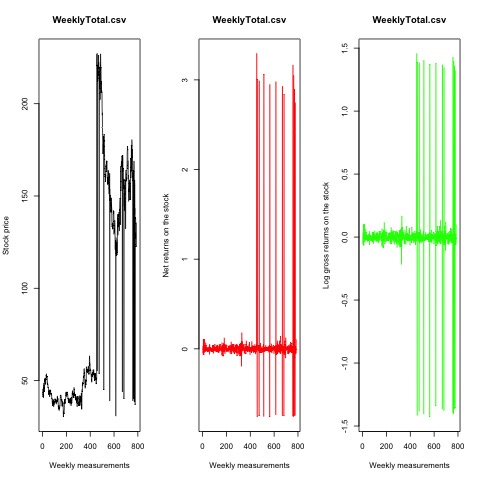
\includegraphics[scale = 0.4]{/Users/kimartin/Desktop/PDM_thesis_report/latex_template5_57/main/R_Files_3/WeeklyTotal.jpeg}
     	\caption{15 years of weekly Total Stock Price Data}
     	\label{fig:TotalStock}
	\end{minipage}
\end{figure}
\newpage
\paragraph{}
Let $X_t$ be the price of a stock at time t, the gross return at time t + 1 is defined as the ratio $\frac{X_{t+1}}{X_t}$, the net return at time t + 1 is defined as the ratio $r_t = \frac{X_{t+1}-X_t}{X_t}$ and the log gross return at time t +1 is defined as the log of the gross return at time t + 1 i.e. $R_t = \log(\frac{X_{t+1}}{X_t})$. The latter two quantities are of particular interest in Finance. 
\newline
Let us observe that the relationship between $R_t$, $X_t$ and $X_{t+1}$ can be rewritten as $X_{t+1} = \exp(R_{t+1})*X_t$. An approximation would be to take $X_{t+1} = (1 + R_{t+1})*X_t$ by taking the expansion of the exponential, cut at order 1. Below are the plots of the quantities $\exp(R_t)$ and 1 + $R_t$ for the five stocks previously considered. As we can see from the value of the residuals, this is in practice a very good approximation !
\begin{figure}[h!]
	\centering
	\begin{minipage}[b]{0.4\textwidth}
		\centering
		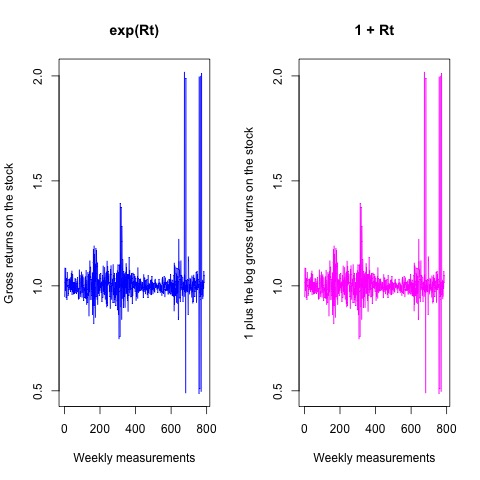
\includegraphics[scale = 0.4]{/Users/kimartin/Desktop/PDM_thesis_report/latex_template5_57/main/R_Files_3/WeeklyBNP_1+Rt_eRt.jpeg}
		\caption{$\exp(R_t)$ and 1 + $R_t$ for BNP Stock Price Data, residual : 3.22E-15}
		\label{fig:BNPCompApproxStock}
	\end{minipage}
	~
	\begin{minipage}[b]{0.4\textwidth}
		\centering
		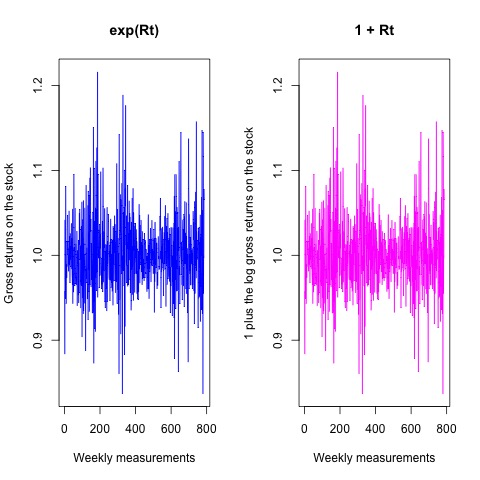
\includegraphics[scale = 0.4]{/Users/kimartin/Desktop/PDM_thesis_report/latex_template5_57/main/R_Files_3/WeeklyCarrefour_1+Rt_eRt.jpeg}
		\caption{$\exp(R_t)$ and 1 + $R_t$ for Carrefour Stock Price Data, residual : 1.44E-15}
		\label{fig:CarrefourCompApproxStock}
	\end{minipage}
\end{figure}
\begin{figure}[h!]
	\centering
	\begin{minipage}[b]{0.4\textwidth}
		\centering
		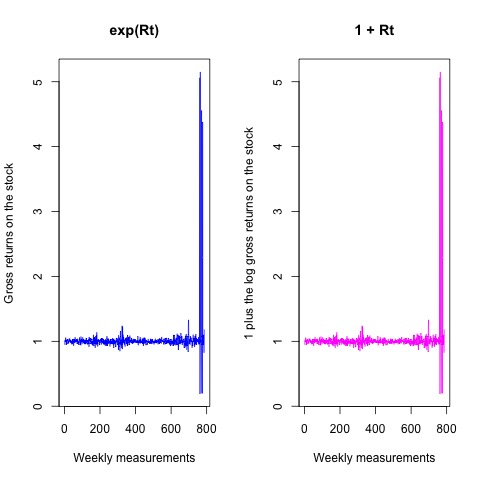
\includegraphics[scale = 0.4]{/Users/kimartin/Desktop/PDM_thesis_report/latex_template5_57/main/R_Files_3/WeeklyLVMH_1+Rt_eRt.jpeg}
		\caption{$\exp(R_t)$ and 1 + $R_t$ for LVMH Stock Price Data, residual : 4.75E-15}
		\label{fig:LVMHCompApproxStock}
	\end{minipage}
	~
	\begin{minipage}[b]{0.4\textwidth}
		\centering
		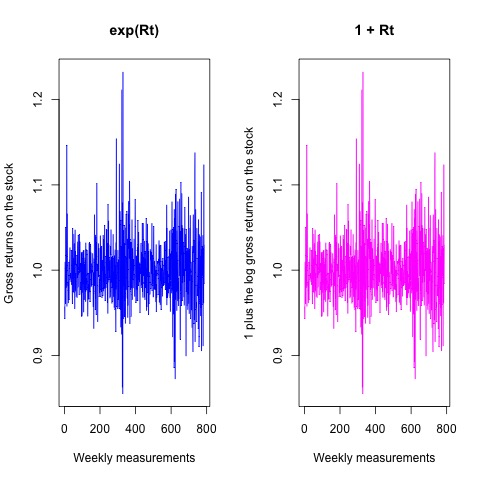
\includegraphics[scale = 0.4]{/Users/kimartin/Desktop/PDM_thesis_report/latex_template5_57/main/R_Files_3/WeeklySanofi_1+Rt_eRt.jpeg}
		\caption{$\exp(R_t)$ and 1 + $R_t$ for Sanofi Stock Price Data, residual : 1.55E-15}
		\label{fig:SanofiCompApproxStock}
	\end{minipage}
	~
	\begin{minipage}[b]{0.4\textwidth}
		\centering
		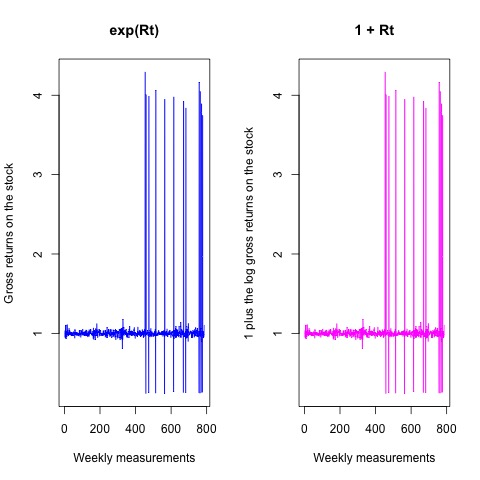
\includegraphics[scale = 0.4]{/Users/kimartin/Desktop/PDM_thesis_report/latex_template5_57/main/R_Files_3/WeeklyTotal_1+Rt_eRt.jpeg}
		\caption{$\exp(R_t)$ and 1 + $R_t$ for Total Stock Price Data, residual : 3.86E-15}
		\label{fig:TotalCompApproxStock}
	\end{minipage}
\end{figure}
\paragraph{}

\newpage
\section{A détour around Brownian Motion}
\section{Back to the data}



